\subsection{Developing prototypes}
When designing a product multiple approaches can be taken.  
UCD aims to increase effectiveness, accessibility, and sustainability, as well as increase the pleasure the user experiences when using the system\cite{user-centred-design}. 
An alternative to UCD is LeanUX \cite{Lean_UX}.
Lean UX is also a user centered approach for UX development that is often used in start-ups.
The approach focusses on creating minimal viable products(MVPs) that can be iteratively released and tested with representative users.

In this project, the stakeholder has suggested that we based our design on existing solutions.
Therefore, we endeavor towards a design strategy where we base the design on the current state-of-the-art systems for meeting-management and preferences of the stakeholder.

To develop the prototypes, the sketching tool Figma is used \cite{Figma}.
Figma can be used to design both high- and low-fidelity prototypes, which enables the designer to easily create a lofi prototype, and then later refine it such that users can interact with it.
Figma contains a rich set of user interface components that can be used and modified when creating prototypes.
When a user interacts with a hifi prototype, by, for instance, clicking a UI element, the designer can enable a transition to a different view, thus simulating system UI behavior.
Based on the initial interviews described in Section \ref{sec:understanding_the_problem}, the prototypes must be suitable for use on a simple monitor, such as a tablet.

During this project, both a lofi and hifi prototype has been developed.
Each prototype shows a UI highlighting two situations for meeting rooms. 
Each situation depicts different states of a meeting room (occupied or available) which allows us to explore how users want to interact with the system in these different situations. 

The development of a lofi prototype has been used as an internal exercise, independent from stakeholders, to explore initial design ideas based on existing systems.
Figure \ref{fig:lofi_prototype} depicts two views from the prototype, each based on the current state of the meeting room.
Depending on the state of the room, the background color as well as the actions available for the user changes.
Figure \ref{fig:lofi_prototype:a} depicts a view shown when a meeting is occupied.
Here, the main action available is to end the current meeting.
Figure \ref{fig:lofi_prototype:b} depicts a view shown when a meeting room is available.
From this view, the main action is to book the meeting room.

\begin{figure}
    \centering
    \begin{subfigure}[b]{0.49\textwidth}
        \centering
        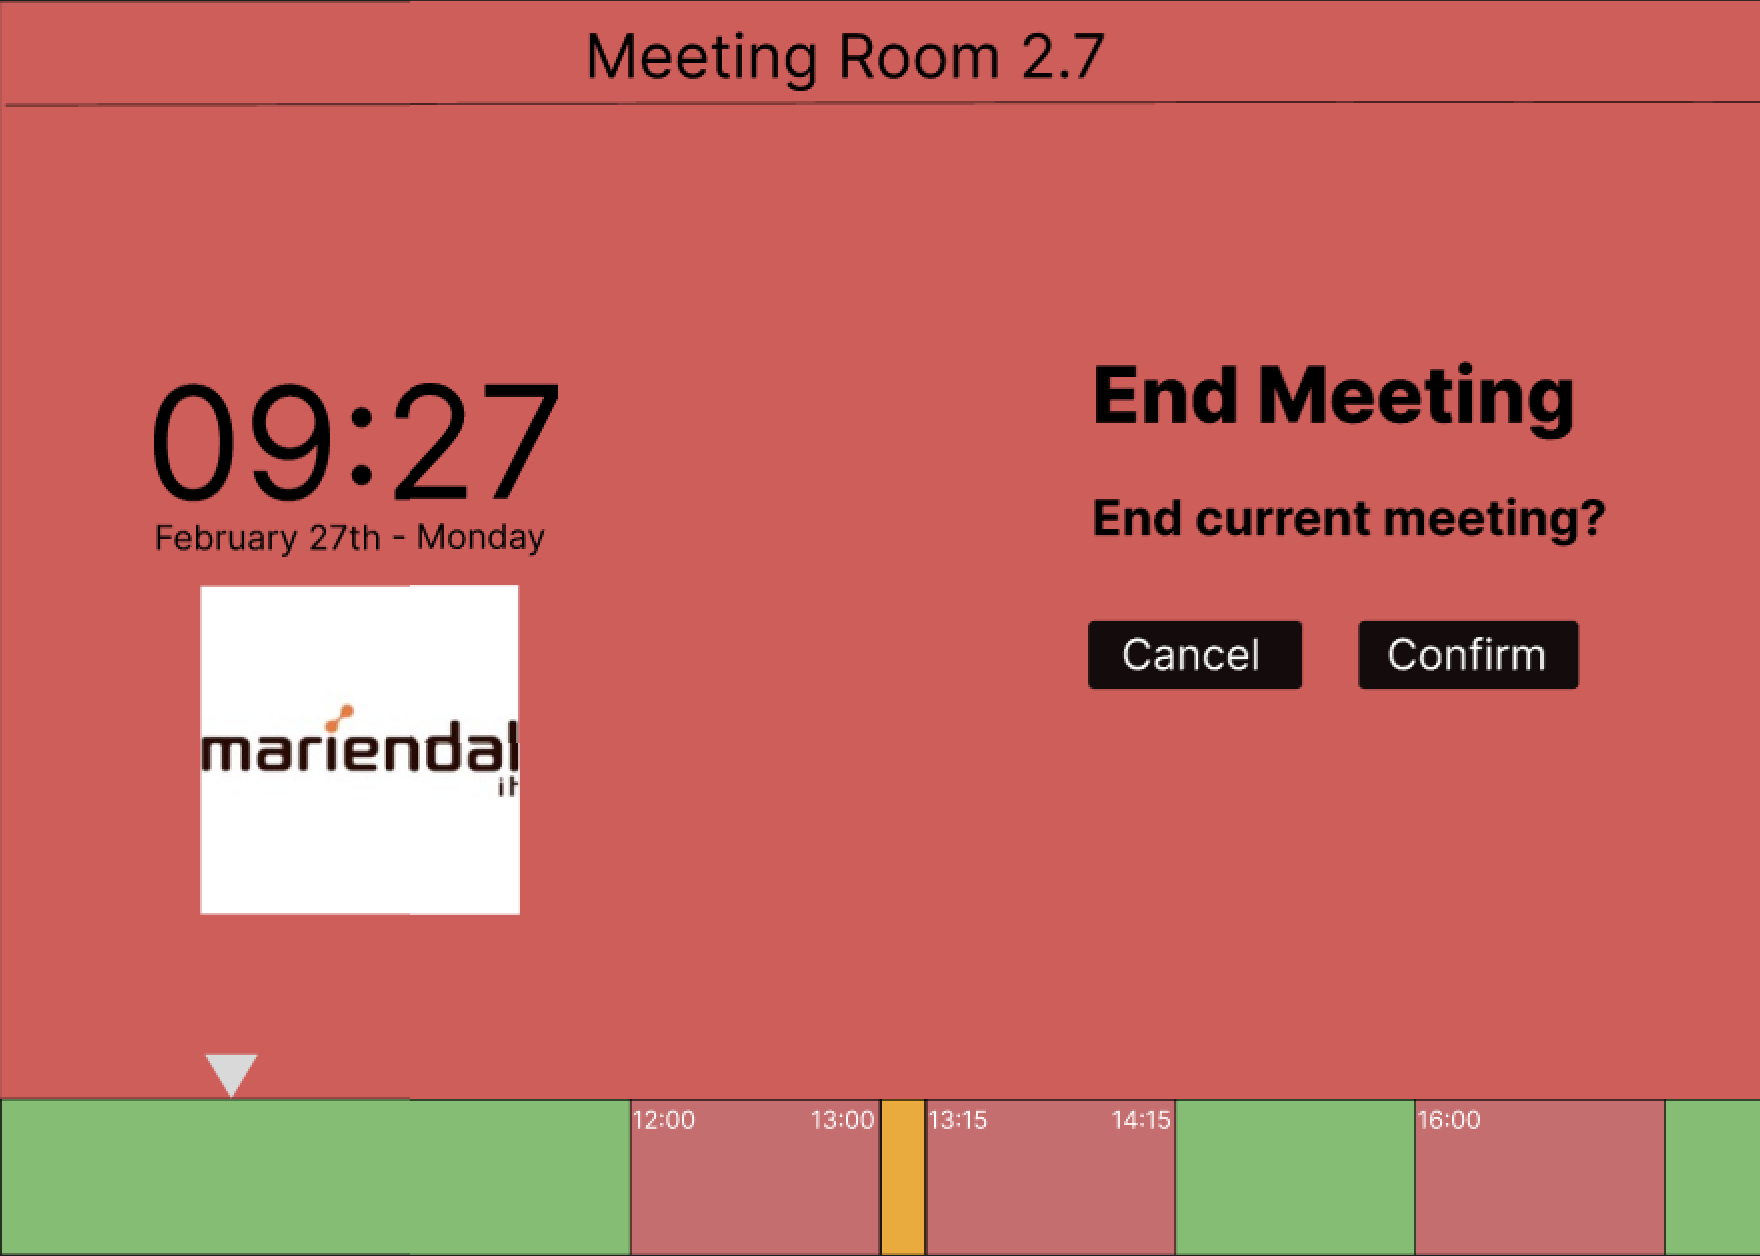
\includegraphics[width=\textwidth]{images/lofi_end.png}
        \caption{Tablet view for when a meeting room is occupied.}
        \label{fig:lofi_prototype:a}
    \end{subfigure}
    \begin{subfigure}[b]{0.49\textwidth}
        \centering
        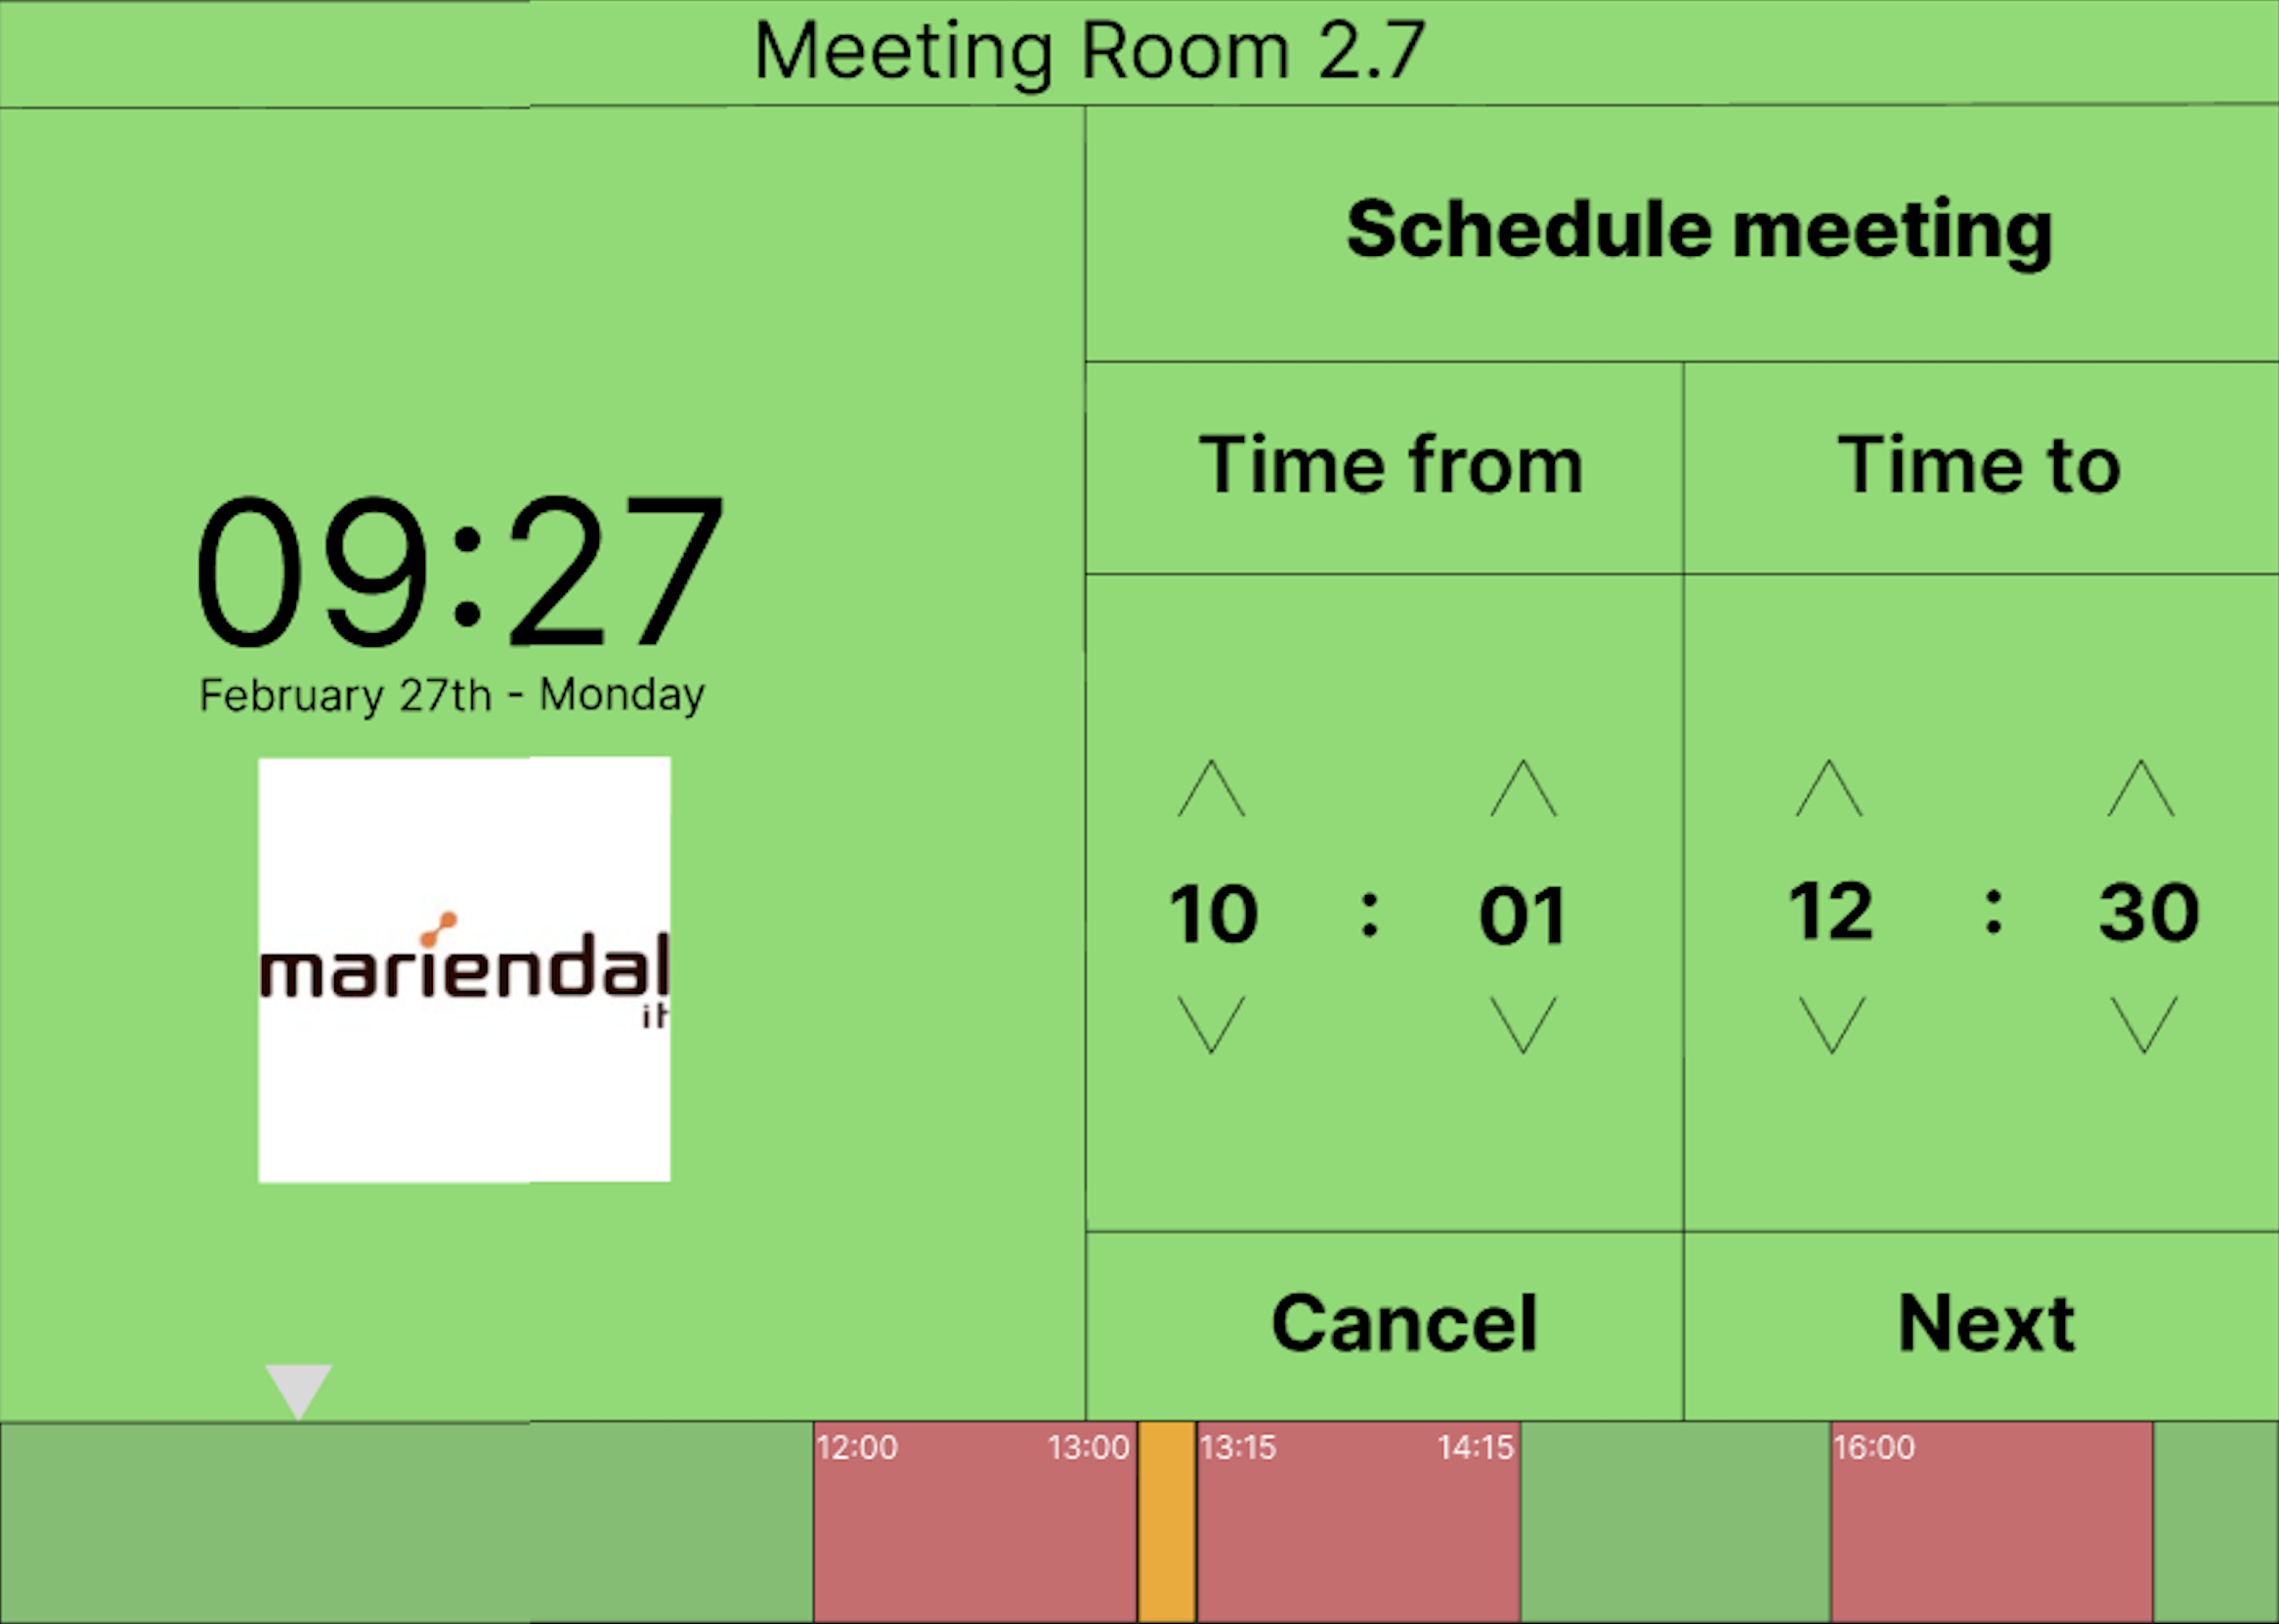
\includegraphics[width=\textwidth]{images/lofi_schedule.png}
        \caption{Tablet view for when a meeting room is available}
        \label{fig:lofi_prototype:b}
    \end{subfigure}
    \caption{Two views of the low fidelity prototype, each enabling different actions based on the state of the meeting room.}
    \label{fig:lofi_prototype}
\end{figure}

Based on this prototype, multiple ideas for an hifi prototype was conceived.
These ideas were filtered and selected upon, and turned into a hifi prototype.

Figure xxxx depicts the views for the same situations shown in Figure \ref{fig:lofi_prototype}, where a room is either occupied or available.
The hifi prototype enables user interaction with all elements that would be interactive in a final design.
Each user interaction with an interactive element leads the user to a different view, as depicted in Figure xxx. %a subfigure that explains that when botton x is clicked the user is taken to view X
All views for the hifi prototype can be found in Appendix xxxx. 

\subsubsection{Developing a high fidelity prototype}
Figure xx depicts the main view of a room is occupied.